\documentclass[12pt,oneside]{article}

%%%%%%%%%%%%%%%%%%%%%%%%%%%%
%%   Zusaetzliche Pakete  %%
%%%%%%%%%%%%%%%%%%%%%%%%%%%%
\usepackage{acronym}
\usepackage{enumerate}
\usepackage{a4wide}
\usepackage{fancyhdr}
\usepackage[pdftex]{graphicx}
\usepackage{palatino}
\usepackage{blindtext}
\usepackage{multirow}
\usepackage[ruled,longend]{algorithm2e}
\usepackage{float}
\usepackage{amsmath}
\usepackage{amssymb}
\usepackage{listings}
\usepackage[numbib]{tocbibind}

%folgende Zeile auskommentieren für englische Arbeiten
\usepackage[ngerman]{babel}

%folgende zeile auskommentieren und die darunter verwenden, um die link-border zu verbergen
%\usepackage[bookmarks]{hyperref}
\usepackage[bookmarks,hidelinks]{hyperref}
\usepackage[T1]{fontenc}
\usepackage[utf8]{inputenc}
\usepackage[a-1b]{pdfx}
\usepackage[justification=centering]{caption}
%\usepackage[style=unsrt,natbib=true,backend=biber]{biblatex}
\usepackage{csquotes}
\usepackage{url}
%\usepackage{subfigure}
\usepackage[utf8]{inputenc}
\usepackage[T1]{fontenc}
% Layout corrections (Schusterjungen)
\clubpenalty = 10000
% Layout corrections (Hurenkinder)
\widowpenalty = 10000
\displaywidowpenalty = 10000

% Figures
\usepackage{caption}
\usepackage[hypcap=true,labelformat=simple]{subcaption}
\renewcommand{\thesubfigure}{(\alph{subfigure})}

% Tables
\usepackage{booktabs}

% Newcommand TODO (red in text)
\newcommand{\todo}[1]{\textcolor{red}{TODO: #1}}

% Newcommand TODOM (red at border)
\newcommand{\todom}[1]{\marginpar{\parbox{1.5cm}{\textcolor{red}{TODO:\\ #1}}}}

% Format für dd.mm.yyy format
\newcommand{\todayddmmyyyy}{%
    \ifnum
        \day<10 0
    \fi\the\day.%
    \ifnum
        \month<10 0
    \fi\the\month.%
    \the\year}


%%%%%%%%%%%%%%%%%%%%%%%%%%%%%%
%% Definition der Kopfzeile %%
%%%%%%%%%%%%%%%%%%%%%%%%%%%%%%

\pagestyle{fancy}
\fancyhf{}
\cfoot{\thepage}
\setlength{\headheight}{16pt}

%%%%%%%%%%%%%%%%%%%%%%%%%%%%%%%%%%%%%%%%%%%%%%%%%%%%%
%%  Definition des Deckblattes und der Titelseite  %%
%%%%%%%%%%%%%%%%%%%%%%%%%%%%%%%%%%%%%%%%%%%%%%%%%%%%%

\newcommand{\HSFTitle}[8]{

    \thispagestyle{empty}
    \begin{center}
    
\includegraphics[width=0.9\textwidth]{logo_new_2.png} \\
    \vspace*{\stretch{1}}
    \end{center}

    %\vspace*{\stretch{1}}
    {\parindent0cm
    \rule{\linewidth}{.7ex}}
    \begin{center}
    \vspace*{\stretch{1}}
    \sffamily\bfseries\Huge
    #1\\
    \vspace*{\stretch{1}}
    \sffamily\bfseries\large
    #3
    \vspace*{\stretch{1}}
    \end{center}
    \rule{\linewidth}{.7ex}

    \vspace*{\stretch{2}}
    \begin{center}
    \Large #2 am #5 der HS Fulda \\
    \vspace*{\stretch{1}}

    \large Matrikelnummer: #4 \\[1mm]
    \large Erstbegutachtung: #7 \\[1mm]

    \vspace*{\stretch{1}}
    \large Eingereicht am #6
    \end{center}
}


%%%%%%%%%%%%%%%%%%%%%%%%%%%%
%%  Beginn des Dokuments  %%
%%%%%%%%%%%%%%%%%%%%%%%%%%%%

\begin{document}

    \HSFTitle
    {Dokumentation und Versionskontrolle in der Softwareentwicklung bei Grenzebach BSH}        % Titel der Arbeit
    {Hausarbeit} % Typ der Arbeit
    {Luca Michael Schmidt}          % Vor- und Nachname der Autor*in
    {1540963}
    {Fachbereich AI}  % Name des FBs
    {\todayddmmyyyy}        % Tag der Abgabe
    {Prof. Dr.-Ing. J. Konert}     % Name der Erstgutachter*in

    \clearpage

    \lhead{}
    \pagenumbering{Roman}
    \setcounter{page}{1}

    \newpage
\begin{otherlanguage}{ngerman}
\thispagestyle{empty}
\section*{Sperrvermerk}
\thispagestyle{empty}
Die vorliegende Arbeit beinhaltet interne vertrauliche Informationen der Firma ”Gren-
zebach BSH GmbH”. Die Weitergabe des Inhalts der Arbeit und Daten im Gesamten
oder in Teilen ist grundsätzlich untersagt.
Es dürfen keinerlei Kopien oder Abschrif-
ten - auch in digitaler Form - gefertigt werden.
Ausnahmen bedürfen der schriftlichen
Genehmigung der Firma Grenzebach BSH GmbH.
\vspace{4\baselineskip}\\
\end{otherlanguage}

    \clearpage
    \tableofcontents
    \clearpage

    %\addcontentsline{toc}{section}{\listfigurename}
    \listoffigures
    \clearpage


%%%%%%%%%%%%%%%%%%%%%%%%%%%%
%%  Einstellungen  %%
%%%%%%%%%%%%%%%%%%%%%%%%%%%%
    \cleardoublepage
    \pagenumbering{arabic}
    \setcounter{page}{1}
    \lhead{\nouppercase{\leftmark}}

%%%%%%%%%%%%%%%%%%%%%%%%%%%%
%%  Hauptteil  %%
%%%%%%%%%%%%%%%%%%%%%%%%%%%%

%% ---- %%


    \section{Einleitung}
    \label{sec:einleitung}

    \subsection{Relevanz von Dokumentation und Versionskontrolle}
    \label{subsec:relevanz}
    Als essenzielle Bestandteile moderner Softwareentwicklung erhöhen die systematische Dokumentation und konsequente Versionskontrolle die Effizienz von Entwicklungsteams, verbessern die Softwarequalität und ermöglichen eine langfristige Planbarkeit von Wartung und Weiterentwicklung. So reduziert eine aktuelle und verständliche Dokumentation nicht nur den Zeitaufwand für die Informationssuche, sondern beugt auch Fehlern vor, die zu unerwartetem Mehraufwand führen können \cite{webmakers2024}. Darüber hinaus dienen dokumentierte Anforderungen als fundierte Diskussions- und Entscheidungsgrundlage, wodurch die Kommunikation im Team, insbesondere in agilen Kontexten, gefördert wird \cite{fraunhoferIESE2020}. Gleichzeitig sichert die Versionskontrolle den aktuellen Arbeitsstand und erlaubt durch Branching und Merging eine parallele Feature-Entwicklung, was den Entwicklungsprozess maßgeblich beschleunigt \cite{moldstud2024}. In der Praxis zeigt sich, dass Teams, die Versionskontrollsysteme effektiv nutzen, tendenziell weniger Fehler produzieren und diese schneller beheben. Insbesondere in Kontexten mit schnellen Iterationen und kontinuierlicher Auslieferung sind diese Praktiken unverzichtbar, da sie die notwendige Stabilität und Nachvollziehbarkeit gewährleisten.

    \subsection{Unternehmenskontext: Grenzebach BSH im Überblick}
    \label{subsec:unternehmenskontext}
    Die Grenzebach BSH GmbH mit Sitz in Bad Hersfeld ist als Teil der international agierenden Grenzebach-Gruppe ein globaler Spezialist für Anlagenbau und Automatisierungstechnik. Das 1960 gegründete Unternehmen beschäftigt weltweit rund 1.600 Mitarbeiter an sieben Standorten und ist in über 55 Ländern aktiv \cite{GrenzebachWebsite}. Der Schwerpunkt der Grenzebach BSH liegt in der Entwicklung und Fertigung von Industrieanlagen für die Baustoffe Gips und Holz. Neben der in diese Anlagen integrierten Steuerungssoftware gewinnt die Entwicklung von ergänzenden Softwareerweiterungen, spezialisierten Industrie-Apps und unterstützenden Softwarelösungen zunehmend an Bedeutung. Die für diese Softwareentwicklungsprojekte etablierten Dokumentations- und Versionsverwaltungsprozesse stehen im Zentrum der vorliegenden Arbeit.

    \subsection{Zielsetzung und Aufbau der Arbeit}
    \label{subsec:zielsetzung}
    Da bei Grenzebach BSH Optimierungspotenziale in den Prozessen der Dokumentation und Versionskontrolle bestehen, analysiert diese Hausarbeit die gegenwärtigen Praktiken, identifiziert deren Schwachstellen und entwickelt auf dieser Basis konkrete Handlungsempfehlungen.
    \newline
    Die Arbeit ist wie folgt aufgebaut: Kapitel \ref{sec:grundlagen} legt zunächst die theoretische Basis, indem es grundlegende Konzepte, Methoden und aktuelle Standards der Dokumentation und Versionskontrolle vorstellt. Anschließend erfolgt eine detaillierte Ist-Analyse der Prozesse bei Grenzebach BSH. Hierbei untersucht Kapitel \ref{sec:analyse_dokumentation} die Dokumentationspraxis, während Kapitel \ref{sec:evaluation_versionskontrolle} die Versionskontrollprozesse evaluiert. Beide Kapitel identifizieren die jeweiligen Stärken sowie Schwächen und vergleichen die Praktiken mit gängigen Branchenstandards. Darauf aufbauend präsentiert Kapitel \ref{sec:optimierung} spezifische Optimierungsvorschläge und Handlungsempfehlungen für beide Bereiche. Abschließend fasst Kapitel \ref{sec:fazit} die wesentlichen Ergebnisse zusammen, reflektiert diese kritisch und gibt einen Ausblick auf mögliche nächste Schritte.

%% ---- %%


    \section{Theoretische Grundlagen}
    \label{sec:grundlagen}
    Dieses Kapitel erläutert die zentralen Konzepte, Methoden und Werkzeuge der Softwaredokumentation und Versionskontrolle. Es schafft somit das notwendige Fundament für die spätere Analyse und die Entwicklung von Optimierungsvorschlägen.

    \subsection{Dokumentation in der Softwareentwicklung}
    \label{subsec:dokumentation}
    Die Softwaredokumentation umfasst sämtliche schriftlichen und grafischen Materialien, die während des gesamten Softwarelebenszyklus erstellt werden, um das Softwaresystem, dessen Entwicklungsprozess sowie seine Nutzung zu beschreiben. Als integraler Bestandteil der Softwareentwicklung ist sie entscheidend für den Erfolg, die Qualität und die langfristige Wartbarkeit eines Projekts. Zu ihren primären Zielen gehören die effektive Kommunikation innerhalb des Teams und mit externen Stakeholdern, die strukturierte Wissensspeicherung für Teamwechsel und Onboarding sowie die Qualitätssicherung durch klare Spezifikationen und nachvollziehbare Entwicklungsschritte \cite{webmakers2024}. Zusätzlich unterstützt eine sorgfältige Dokumentation die Wartung und Weiterentwicklung bestehender Systeme und dient der Erfüllung vertraglicher oder regulatorischer Anforderungen.
    \newline
    Grundsätzlich wird zwischen Prozess- und Produktdokumentation unterschieden. Während die Prozessdokumentation den Entwicklungsprozess selbst beschreibt (z.B. Projektpläne, Meeting-Protokolle), fokussiert sich die Produktdokumentation auf das zu erstellende oder bereits erstellte Softwaresystem und umfasst verschiedene Artefakte:
    \begin{itemize}
        \item \textbf{Anforderungsdokumentation:} Sie definiert funktionale Anforderungen, oft mittels User Stories oder Use-Case-Diagrammen. Insbesondere in agilen Umfeldern ist sie entscheidend, um Missverständnisse zu vermeiden und eine gemeinsame Produktvision zu entwickeln \cite{fraunhoferIESE2020}.
        \item \textbf{Architektur- und Design-Dokumentation:} Sie beschreibt die Systemstruktur, die einzelnen Komponenten und deren Zusammenspiel. Zudem hält sie Entwurfsentscheidungen fest und dient als wichtiger Leitfaden für die Implementierung.
        \item \textbf{Quellcode-Dokumentation:} Diese umfasst sowohl Code-Kommentare als auch automatisch generierbare API-Dokumentationen, um das Verständnis einzelner Module und Funktionen zu verbessern.
        \item \textbf{Testdokumentation:} Sie beinhaltet Testpläne, Testfallspezifikationen, Testdaten und Testprotokolle, die eine systematische Qualitätsüberprüfung ermöglichen.
        \item \textbf{Benutzerdokumentation:} Mittels Handbüchern, Online-Hilfen oder Tutorials erklärt sie den Endanwendern die Bedienung und Funktionalität der Software.
        \item \textbf{Betriebsdokumentation:} Sie enthält alle notwendigen Informationen für die Installation, Konfiguration und den laufenden Betrieb der Software.
    \end{itemize}
    Typische Herausforderungen bei der Dokumentation sind ihre kontinuierliche Aktualisierung bei sich dynamisch entwickelnden Systemen, das Finden der richtigen Balance zwischen zu viel und zu wenig Information sowie die Förderung von Akzeptanz und konsequenter Nutzung im Team \cite{webmakers2024}. Qualitativ hochwertige Dokumentation zeichnet sich durch eine klare Struktur, zielgruppengerechte Inhalte und etablierte Prozesse zur Qualitätssicherung aus. Die Norm ISO/IEC/IEEE 26514 betont in diesem Zusammenhang die Notwendigkeit von Zielgruppen- und Tätigkeitsanalysen sowie von zielgruppenzentrierten Informationskonzepten \cite{styrz2022normen}.

    \subsection{Versionskontrollsysteme und -prozesse}
    \label{subsec:versionskontrolle}
    Ein Versionskontrollsystem (VCS) ist ein fundamentales Werkzeug in der Softwareentwicklung, das Änderungen an Dateien über die Zeit systematisch protokolliert und verwaltet. Dessen Einsatz ist für eine effektive Teamkoordination, eine lückenlose Änderungshistorie und die Integrität des Quellcodes unerlässlich \cite{ChaconStraubProGit}. Ohne ein VCS drohen Risiken wie das unbeabsichtigte Überschreiben von Änderungen, Schwierigkeiten beim Zusammenführen unterschiedlicher Arbeitsstände oder der unwiderrufliche Verlust funktionierender Versionen \cite{moldstud2024}.
    \newline
    Moderne VCS basieren auf einer Reihe von Kernkonzepten und essenziellen Funktionalitäten. Das Repository dient als zentraler Speicherort, der alle Projektdateien mitsamt ihrer vollständigen Historie enthält. Jede gesicherte Änderung wird als Commit bezeichnet und umfasst nicht nur die geänderten Dateien, sondern auch Metadaten wie Autor und Zeitpunkt sowie eine erläuternde Commit-Nachricht. Sogenannte Branches ermöglichen die parallele Arbeit an neuen Features, eine isolierte Fehlerbehebung oder Experimente, ohne dabei den Hauptentwicklungszweig (\texttt{main} oder \texttt{master}) direkt zu beeinflussen. Die Integration verschiedener Branches erfolgt durch Merge-Vorgänge, während Tags dazu dienen, spezifische Versionsstände für Releases zu markieren. Mittels Diffs lassen sich Unterschiede zwischen Versionen visualisieren, und Rollbacks ermöglichen die gezielte Rückkehr zu früheren Ständen.
    \newline
    Der typische Git-Arbeitszyklus beginnt mit dem initialen Kopieren eines Remote-Repositories (\texttt{git clone}), gefolgt vom Vorbereiten geänderter Dateien für den nächsten Commit (Staging mit \texttt{git add}). Anschließend werden die Änderungen lokal als Commit gespeichert (\texttt{git commit}), an das Remote-Repository übertragen (\texttt{git push}) und schließlich Remote-Änderungen abgerufen und in den lokalen Arbeitsstand integriert (\texttt{git pull} oder \texttt{git fetch} mit \texttt{git merge}).

    \subsection{Aktuelle Standards und Best Practices in der Industrie}
    \label{subsec:standards}
    Um Dokumentation und Versionskontrolle optimal zu nutzen, haben sich in der Industrie vielfältige Standards und Best Practices entwickelt.
    \newline
    Moderne Dokumentationsansätze zielen auf mehr Flexibilität, Aktualität und eine bessere Integration in den Entwicklungsprozess ab. So betonen agile Dokumentationsprinzipien eine ``gerade genug''-Dokumentation, bei der der Fokus auf funktionierender Software und direkter Kommunikation liegt. User Stories mit präzisen Akzeptanzkriterien spielen hierbei oft eine zentrale Rolle \cite{AgileManifestoDe, fraunhoferIESE2020agilMytho}. Der Ansatz ``Documentation as Code'' behandelt Dokumentation wie Softwarequellcode: Sie wird in leichtgewichtigen Markup-Sprachen (z.B. Markdown, AsciiDoc) verfasst, im VCS versioniert, durchläuft Review-Prozesse und kann automatisiert in verschiedene Zielformate überführt werden \cite{WriteTheDocsWhatIsDocsAsCode}.
    \newline
    Im Bereich der Versionskontrollsysteme, insbesondere bei Git, haben sich ebenfalls etablierte Praktiken durchgesetzt. Dies beginnt bei der Wahl eines geeigneten Branching-Modells wie dem stark strukturierten Gitflow oder dem agileren Trunk-Based Development \cite{AtlassianGitWorkflows}. Standardisierte Commit-Nachrichten, beispielsweise nach dem Schema von ``Conventional Commits'', sorgen für eine klare und maschinell auswertbare Historie \cite{ConventionalCommitsOrgDe}. Die Qualitätssicherung des Codes erfolgt durch systematische Code Reviews mittels Pull-Requests, während eine transparente Versionierung durch Semantic Versioning (\texttt{MAJOR.MINOR.PATCH}) gewährleistet wird \cite{AtlassianWasIstEinPullRequest, SemVerOrgDe}. Die nahtlose Integration in CI/CD-Pipelines ermöglicht darüber hinaus eine effiziente und zuverlässige Auslieferung der Software.

    \subsection{Relation zwischen Dokumentation und Versionskontrolle}
    \label{subsec:relation}
    In der modernen Softwareentwicklung sind Dokumentation und Versionskontrolle eng miteinander verzahnt und entfalten im Zusammenspiel erhebliche Synergien. Die Verwaltung von Dokumentationsartefakten in einem VCS ist insbesondere für den ``Documentation as Code''-Ansatz von zentraler Bedeutung, da textbasierte Dokumente hierbei gemeinsam mit dem Quellcode versioniert werden. Durch den Einsatz von Branching und Merging können Dokumentationsänderungen parallel zu den zugehörigen Code-Features entwickelt und mittels Pull-Requests gemeinsam einem Review unterzogen werden, was sowohl die Konsistenz als auch die Nachvollziehbarkeit sicherstellt.
    \newline
    Zudem dienen aussagekräftige Commit-Nachrichten, die idealerweise Standards wie ``Conventional Commits'' \cite{ConventionalCommitsOrgDe} folgen, als eine Art granulare Dokumentation der Änderungshistorie. Moderne Entwicklungsplattformen ermöglichen es darüber hinaus, Dokumentation direkt mit spezifischen Features oder Issues zu verknüpfen, was das Auffinden kontextbezogener Informationen erheblich erleichtert.
    \newline
    Diese integrierte Nutzung verbessert letztlich die Wartbarkeit, Qualität und Transparenz von Softwareprojekten und erleichtert zudem das Onboarding neuer Teammitglieder. VCS-gestützte Prozesse, bei denen Dokumentationsanpassungen im selben Zyklus wie Code-Änderungen behandelt werden, lösen die klassische Herausforderung, die Synchronisation zwischen dynamischem Code und aktueller Dokumentation zu gewährleisten. Diese Synergieeffekte werden in den folgenden Kapiteln bei der Analyse der Praxis bei Grenzebach BSH von besonderer Relevanz sein.

%% ---- %%


    \section{Analyse der Dokumentationspraxis bei Grenzebach BSH}
    \label{sec:analyse_dokumentation}
    Dieses Kapitel untersucht detailliert die aktuelle Praxis der Erstellung, Verwaltung und Nutzung von Softwaredokumentation bei Grenzebach BSH. Ziel ist es, ein klares Bild der etablierten Prozesse und eingesetzten Werkzeuge zu zeichnen, um darauf aufbauend Stärken, Schwächen und Optimierungspotenziale zu identifizieren.

    \subsection{Aktuelle Vorgehensweisen und Werkzeuge}
    \label{subsec:dokument_werkzeuge}
    Die Dokumentationspraxis für Softwareprojekte bei Grenzebach BSH basiert auf einer zweigeteilten Strategie, die sich primär an interne Entwicklerteams richtet: Sie nutzt Confluence für übergreifende Projektinformationen und GitHub für die technische sowie code-nahe Dokumentation.
    \newline
    Für die übergeordnete und konzeptionelle Dokumentation neuer Projekte werden in Confluence Projektseiten nach standardisierten Vorlagen angelegt. Diese Seiten dienen als zentrale Ablage für verschiedenste Artefakte, darunter textuelle Beschreibungen, DrawIO-Grafiken und -Diagramme, Screenshots, Click-Dummies, Prototypen, Wireframes, Interface-Spezifikationen sowie Besprechungsnotizen. Die Erstellung und Pflege dieser Inhalte erfolgen kollaborativ durch mehrere Teammitglieder, wobei das jeweils verantwortliche Mitglied die Richtigkeit und Qualität durch Proofreading sicherstellt. Obwohl nicht immer, ist die Dokumentation gelegentlich Bestandteil wöchentlicher Scrum-Meetings, in denen Verbesserungen und Aktualisierungen diskutiert werden.
    \newline
    Die technische Dokumentation ist hingegen eng mit GitHub und den CI/CD-Prozessen via GitHub Actions verknüpft. Jedes Projekt pflegt einen spezifischen ``Doc-Branch'' im Repository, der HTML-Dateien und eingebundene JSON-Daten als automatisch generierte technische Dokumentation enthält. Nach einer Vorlage erstellte \texttt{README.md}-Dateien, die grundlegende Projektinformationen wie Zweck, Nutzung, Installation und Besonderheiten zusammenfassen, werden ebenfalls ins HTML-Format überführt und integriert. GitHub Actions aktualisieren zudem automatisch Badges in den \texttt{README.md}-Dateien, um den aktuellen Versionsstand, Testergebnisse und den Sicherheitsstatus anzuzeigen. Die so generierte Dokumentation, die auch aus dem Quellcode extrahierte Kommentare und Kontextinformationen umfasst, wird auf einem internen Server publiziert. Bei besonders komplexen Sachverhalten verlinkt sie bei Bedarf direkt zu detaillierteren Confluence-Seiten. Die grundlegendste Ebene der Dokumentation bilden jedoch stets die Code-Kommentare, die von den Entwicklern direkt im Code verfasst werden.
    \newline
    Zusammenfassend verfolgt Grenzebach BSH einen zweigeteilten Ansatz: Confluence fungiert als Wissensbasis für umfassende, grafisch-konzeptionelle Projektinformationen, die kollaborativ erstellt und regelmäßig besprochen werden. GitHub bildet das Zentrum für eine technische, versionskontrollierte Dokumentation, die teilweise automatisiert generiert, durch CI/CD-Prozesse aktuell gehalten und bei Bedarf mit Confluence verknüpft wird. Diese Aufteilung spiegelt die in Abschnitt \ref{subsec:dokumentation} beschriebenen unterschiedlichen Dokumentationsarten wider.

    \subsection{Stärken und Schwächen der bisherigen Praxis}
    \label{subsec:ss_dok}
    Die Analyse der Dokumentationspraxis bei Grenzebach BSH offenbart sowohl etablierte Stärken als auch Bereiche mit erkennbaren Herausforderungen und Optimierungspotenzialen.
    \newline
    Zu den Stärken zählt die klare Aufgabenteilung zwischen Confluence für übergreifende Informationen und GitHub für die code-nahe Dokumentation, wobei Confluence als zentrale Ablage für modulübergreifende Artefakte dient. Die Verwendung von Vorlagen in Confluence stellt einen wichtigen ersten Schritt in Richtung Einheitlichkeit dar. Ein weiterer positiver Aspekt ist die automatische HTML-Generierung und die Integration von Status-Badges in den \texttt{README.md}-Dateien, was Entwicklern eine schnell erfassbare Projektübersicht bietet und das Team motiviert, diese Indikatoren positiv zu halten. Ebenso wird die Möglichkeit, von Code-Kommentaren auf erläuternde Confluence-Inhalte zu verlinken, als hilfreich für das Verständnis komplexer Zusammenhänge empfunden. Diese automatisierten Prozesse entsprechen bereits in Teilen dem in Abschnitt \ref{subsec:standards} beschriebenen ``Documentation as Code''-Ansatz.
    \newline
    Demgegenüber stehen jedoch auch Schwächen und Herausforderungen. Die Aufteilung der Dokumentation auf Confluence und GitHub führt trotz Verlinkungen zu potenziellen Synchronisationsproblemen, da keine automatisierte Abgleichung stattfindet. Dies kann zu Inkonsistenzen wie veralteten Code-Kommentaren, \texttt{README.md}-Dateien, Confluence-Seiten oder toten Links führen \cite{webmakers2024}. Es fehlen klare Regeln, welche Informationsquelle als führend gilt, auch wenn tendenziell Confluence für allgemeine und GitHub für code-spezifische Inhalte genutzt wird. Zudem variiert die Qualität der Code-Kommentare stark je nach Teammitglied. Obwohl Confluence-Seiten generell gut gepflegt sind, bleibt deren kontinuierliche Aktualisierung eine stetige Herausforderung. Die Thematisierung der Dokumentation in Scrum-Meetings fokussiert sich häufig auf Tests, und nicht alle Teammitglieder zeigen das gleiche Engagement für Dokumentationsaufgaben, sodass wichtige Aspekte teilweise auch auf Rückfrage hin nicht ergänzt werden. Schließlich fehlt eine vollständige Abdeckung aller in Abschnitt \ref{subsec:dokumentation} genannten Dokumentationsarten, insbesondere für Endanwender, während andere Bereiche gut versorgt sind.

    \subsection{Vergleich mit Branchenstandards}
    \label{subsec:vergleich_dok}
    Der Vergleich der bei Grenzebach BSH etablierten Praxis mit den in Kapitel \ref{sec:grundlagen} dargestellten Branchenstandards zeigt sowohl fortschrittliche Ansätze als auch deutliche Weiterentwicklungspotenziale.
    \newline
    Positiv hervorzuheben sind die auf GitHub Actions basierende HTML-Generierung, die Versionierung der Dokumentation in einem dedizierten ``Doc-Branch'' und die Extraktion von Code-Kommentaren. Diese Aspekte setzen bereits wesentliche Elemente des ``Documentation as Code''-Prinzips um \cite{WriteTheDocsWhatIsDocsAsCode}. Die automatische Generierung aus dem reviewten \texttt{develop}-Branch ohne manuelle Zwischenschritte fördert die Konsistenz, und die Nutzung von \texttt{README.md}-Dateien mit automatisierten Status-Badges entspricht modernen Praktiken. Darüber hinaus unterstützt die regelmäßige Besprechung der Dokumentation in Scrum-Meetings agile Grundsätze \cite{AgileManifestoDe, fraunhoferIESE2020agilMytho}. Die einheitliche Verwendung von DrawIO für Diagramme in Confluence ist ebenfalls positiv zu bewerten. Diese Praktiken zeigen, dass Grenzebach BSH bereits wichtige Elemente moderner Dokumentationsstrategien erfolgreich implementiert hat.
    \newline
    Optimierungspotenzial zeigt sich jedoch in der Durchgängigkeit des ``Documentation as Code''-Ansatzes. Werkzeuge wie Sphinx oder MkDocs, die Markdown oder AsciiDoc direkt aus dem Haupt-Repository verarbeiten, könnten den separaten ``Doc-Branch'' überflüssig machen und eine noch engere Verzahnung mit dem Code ermöglichen. Dies würde Review-Prozesse vereinfachen, da Dokumentationsänderungen im selben Diff wie die zugehörigen Code-Änderungen sichtbar wären. Während die Bereitstellung der HTML-Dokumentation auf einem internen Webserver funktional ist, könnte sie durch integrierte Lösungen wie GitHub-Wiki-Funktionen oder spezialisierte Doku-Hosting-Plattformen weiter optimiert werden.
    \newline
    Die Trennung der Dokumentation auf Confluence und GitHub-generierte Seiten weicht vom Ideal einer ``Single Source of Truth'' ab, solange klare Prozesse zur Definition der führenden Quellen und zur Sicherung der Aktualität fehlen \cite{webmakers2024}. Die stark variierende Dokumentationsqualität je nach Teammitglied deutet zudem auf das Fehlen verbindlicher Richtlinien hin, während eine systematische Qualitätssicherung, die über einfaches Proofreading hinausgeht und sich an Normen wie ISO/IEC/IEEE 26514 orientiert \cite{styrz2022normen}, noch nicht etabliert ist. Eine automatisierte Überprüfung der Verlinkungen zwischen Confluence und GitHub wäre eine konkrete Annäherung an Best Practices für wartbare Dokumentationssysteme. Diese Erkenntnisse bilden die Grundlage für die in Kapitel \ref{sec:optimierung} entwickelten Verbesserungsvorschläge.

%% ---- %%


    \section{Evaluation der Versionskontrolle bei Grenzebach BSH}
    \label{sec:evaluation_versionskontrolle}
    Nach der Analyse der Dokumentationspraxis widmet sich dieses Kapitel der detaillierten Evaluation der Versionskontrollsysteme und der damit verbundenen Workflows bei Grenzebach BSH. Ziel ist es, die aktuellen Prozesse zu beschreiben, deren Stärken und Schwächen zu identifizieren und sie mit gängigen Branchenstandards zu vergleichen.

    \subsection{Eingesetzte Versionskontrollsysteme und Workflows}
    \label{subsec:vk_systeme}
    Die Versionskontrolle bei Grenzebach BSH basiert auf Git, wobei GitHub als zentrale Hosting-Plattform dient. Dieses System wird durch GitHub Actions für CI/CD-Prozesse und Jira für das Projektmanagement ergänzt. Über die in den IDEs (JetBrains, Visual Studio Code) integrierten Funktionen hinaus werden keine speziellen Git-Clients verwendet. Die Nutzung von Git und GitHub ist im Team fest etabliert und wird durchgängig wie vorgesehen umgesetzt.
    \newline
    Die Erstellung neuer Projekte folgt einem standardisierten Prozess: Ein Git-Template wird heruntergeladen und ein zugehöriges Setup-Skript ausgeführt. Dieses Skript generiert die lokale Git-Umgebung, erstellt das Remote-Repository auf GitHub inklusive der notwendigen Zugriffsrechte, legt einen ``Doc-Branch'' an, richtet die GitHub Actions ein und passt die \texttt{README.md} sowie Standarddateien wie \texttt{.gitignore} und \texttt{LICENSE} an. Dieser reibungslose Ablauf spart erheblich Zeit bei der Projekteinrichtung.
    \newline
    Das Branching-Modell ist klar definiert und wird konsequent eingehalten. Der \texttt{develop}-Branch fungiert als Hauptentwicklungszweig. Neue Feature-Branches folgen dem Schema \texttt{GBV-xxx}, welches sich auf die entsprechenden Jira-Tickets bezieht. Releases werden durch Tags im Format \texttt{vx.x.x} markiert. Diese Tags werden manuell gesetzt, woraufhin die CI/CD-Pipeline deren Validität prüft und einen formalen GitHub-Release erstellt. Diese klare Struktur ermöglicht eine nachvollziehbare Entwicklung und unterstützt die in Abschnitt \ref{subsec:versionskontrolle} beschriebenen Kernkonzepte von Versionskontrollsystemen.
    \newline
    Pull Requests (PRs) sind ein zentraler Bestandteil des Workflows. Änderungen aus Feature-Branches werden nicht direkt in den Hauptzweig gemerged, sondern durchlaufen stets einen PR-Prozess. Der Entwickler des Features initiiert den PR, der anschließend ein Code-Review durch mindestens einen Kollegen erfordert, typischerweise eine Person mit Kenntnissen des betreffenden Features. Erst nach Zustimmung erfolgt der Merge in den \texttt{develop}-Branch. Dieser Prozess wird konsequent befolgt.

    Abbildung \ref{fig:git_branching} visualisiert den beschriebenen Git-Workflow mit dem etablierten Branching-Modell und dem integrierten Review-Prozess.

    \begin{figure}[H]
        \centering
        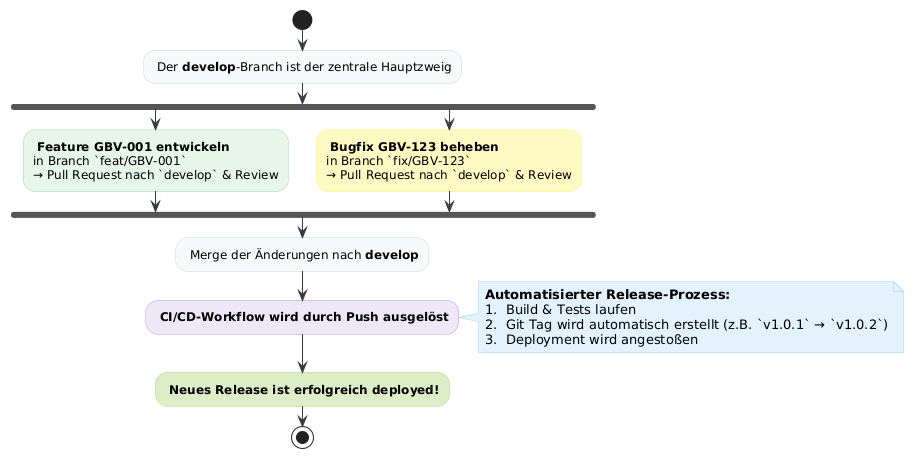
\includegraphics[width=0.85\textwidth]{images/git_branching}
        \caption{Git-Workflow bei Grenzebach BSH: Feature- und Bugfix-Branches (GBV-xxx) durchlaufen einen Pull-Request-Prozess mit Review vor dem Merge in develop. Ein Push auf develop löst automatisch den CI/CD-Workflow und Release-Prozess aus}
        \label{fig:git_branching}
    \end{figure}
    \noindent
    Die Continuous Integration (CI) via GitHub Actions ist an Commits auf dem \texttt{develop}-Branch gekoppelt. Die Pipeline umfasst dabei mehrere Schritte: Extraktion von Projektinformationen und Aktualisierung der \texttt{README.md}, Code-Linting und -Formatierung, eine Sicherheitsprüfung, die Ausführung automatisierter Tests sowie die Generierung der technischen Dokumentation mittels \texttt{pdoc}. Die Rückmeldungen aus der CI-Pipeline sind meist zielführend; bei komplexeren Fehlern ist der für die Pipeline zuständige Entwickler verantwortlich. Diese automatisierten Prozesse unterstützen die in Abschnitt \ref{subsec:dokument_werkzeuge} beschriebene Generierung der technischen Dokumentation.
    \noindent
    Die konkrete Ausgestaltung der CI/CD-Pipeline mit allen automatisierten Schritten und deren Abhängigkeiten zeigt Abbildung \ref{fig:git_workflow}.

    \begin{figure}[H]
        \centering
        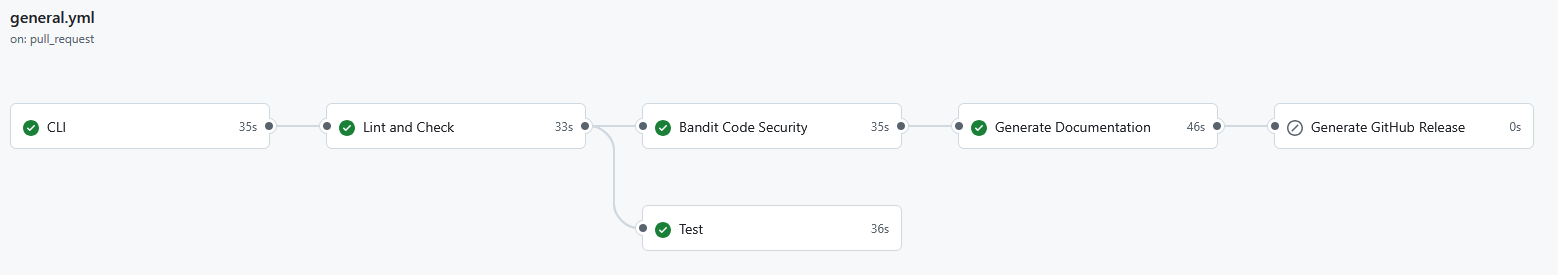
\includegraphics[width=1.0\textwidth]{images/git_workflow}
        \caption{GitHub Actions CI/CD-Pipeline (general.yml) bei Grenzebach BSH: Sequenzielle Ausführung von CLI-Checks, Code-Linting, Sicherheitsprüfung mit Bandit, Tests und Dokumentationsgenerierung mit finaler Release-Erstellung}
        \label{fig:git_workflow}
    \end{figure}

    \noindent
    Das Continuous Deployment (CD) erfolgt ebenfalls über GitHub Actions nach einem erfolgreichen Push auf \texttt{develop} und beinhaltet das Deployment auf einen internen Server. Nach der Erstellung eines Release-Tags wird die Software zudem auf einem internen PyPi-Server bereitgestellt, der sich selbstständig aktualisiert und somit GitHub-unabhängige Bibliotheksinstallationen ermöglicht.
    \newline
    Die Verknüpfung mit Jira erfolgt primär über die Benennung der Branches nach den Ticketnummern (\texttt{GBV-xxx}), was die Nachverfolgbarkeit erleichtert. Eine tiefere, automatisierte Synchronisation zwischen Jira und GitHub, wie beispielsweise automatische Kommentare oder Statusänderungen in Tickets, ist aktuell nicht implementiert; die Information über erstellte PRs erfolgt manuell.

    \subsection{Stärken und Schwächen der aktuellen Prozesse}
    \label{subsec:ss_vk}
    Die Analyse der Versionskontrollprozesse bei Grenzebach BSH zeigt deutliche Stärken, die zu einer effizienten und qualitativ hochwertigen Entwicklung beitragen, aber auch Bereiche mit Optimierungspotenzial.
    \newline
    Zu den wesentlichen Stärken zählt die konsequente Nutzung von Git und GitHub als zentrale Plattform. Der umfassende Funktionsumfang von GitHub, insbesondere die CI/CD-Möglichkeiten über GitHub Actions mit unternehmenseigenen Runnern, wird als vorteilhaft und kosteneffizient empfunden. Die gute Git-Integration in die gängigen IDEs unterstützt zudem einen reibungslosen Workflow. Der standardisierte Prozess zur Projekterstellung mittels Templates und Setup-Skripten spart wertvolle Zeit und sorgt für konsistente Projektstrukturen, was primär für Python-Projekte gilt. Das etablierte Branching-Modell, visualisiert in Abbildung \ref{fig:git_branching}, fördert mit seiner klaren Trennung von Entwicklungs-, Feature- und Release-Zweigen ein stabiles Release-Management und eine organisierte Feature-Entwicklung.
    \newline
    Die weitgehende CI/CD-Automatisierung stellt eine weitere bedeutende Stärke dar. Automatisierte Tests, Linting und Security Checks erhöhen die Code-Qualität und geben den Entwicklern frühes Feedback. Die automatische Generierung der Dokumentation und die Aktualisierung der \texttt{README.md}-Datei mit Status-Badges steigern die Transparenz und Aktualität wichtiger Projektinformationen. Gleichzeitig ist der obligatorische PR-Prozess mit Code-Review ein wichtiger Mechanismus zur Qualitätssicherung und zum Wissenstransfer im Team. Die Entwickler fühlen sich durch die etablierten VCS-Prozesse und die Automatisierung gut unterstützt, während die Wartung der CI/CD-Pipeline bei einem dedizierten Entwickler liegt. Die in Abbildung \ref{fig:git_workflow} gezeigte Pipeline-Struktur verdeutlicht den Grad dieser umfassenden Automatisierung.
    \newline
    Trotz dieser positiven Aspekte existieren auch Schwächen und Herausforderungen. Das Debugging von Fehlern in den GitHub Actions kann sich als komplex und zeitaufwendig erweisen. Die Ausführungsgeschwindigkeit der Tests könnte durch eine stärkere Parallelisierung verbessert werden, wofür jedoch momentan die zeitlichen Ressourcen fehlen. Obwohl sie grundsätzlich als positiv für die Code-Qualität angesehen werden, empfindet das Team die strengen Linting-Regeln gelegentlich als hinderlich.
    \newline
    Im Bereich der Code-Reviews findet zwar stets eine Überprüfung statt, es fehlen jedoch formalisierte Richtlinien oder Checklisten, die über das Kriterium einer erfolgreichen CI-Pipeline hinausgehen. Dies kann zu einer variierenden Tiefe und Qualität der Reviews führen. Insbesondere bei kritischen Änderungen könnte ein einzelner Reviewer zudem unzureichend sein. Die Qualität der Commit-Nachrichten ist ohne verbindliche Regeln nur mittelmäßig, was sich in vagen Nachrichten oder zu umfangreichen Commits äußert.
    \newline
    Ein weiterer Schwachpunkt ist die fehlende tiefere Integration zwischen Jira und GitHub. Eine Automatisierung, wie das Schließen von Tickets bei gemergten PRs, wäre eine sinnvolle Ergänzung. Darüber hinaus wäre eine Funktion zur Erkennung von "toten Links" eine wünschenswerte Verbesserung. Solche Ergänzungen würden die bereits gute Nachverfolgbarkeit, die durch die \texttt{GBV-xxx}-Benennung gewährleistet ist, weiter optimieren.

    \subsection{Vergleich mit Branchenstandards}
    \label{subsec:vergleich_vk}
    Der Abgleich der bei Grenzebach BSH etablierten Prozesse mit den in Abschnitt \ref{subsec:standards} beschriebenen Branchenstandards ermöglicht eine weitere Einordnung und zeigt konkrete Entwicklungsmöglichkeiten auf.
    \newline
    Das praktizierte Branching-Modell kombiniert geschickt Elemente von Gitflow und Trunk-Based Development. Die Trennung zwischen dem \texttt{develop}-Branch und expliziten Release-Tags ähnelt Gitflow und ermöglicht ein stabiles Release-Management. Gleichzeitig vermeidet die zeitnahe Integration von Feature-Branches in \texttt{develop} langlaufende Zweige, was den Prinzipien des Trunk-Based Development entspricht \cite{AtlassianGitWorkflows}. Dieser hybride Ansatz funktioniert im aktuellen Kontext gut, könnte jedoch für extrem schnelle Release-Zyklen an Flexibilität verlieren. Das in Abbildung \ref{fig:git_branching} dargestellte Modell illustriert diese Balance zwischen Stabilität und Agilität.
    \newline
    Die Prinzipien der ``Conventional Commits'' \cite{ConventionalCommitsOrgDe} werden nicht verbindlich umgesetzt. Obwohl sich die Entwickler um aussagekräftige Nachrichten bemühen, fehlt eine einheitliche, maschinell auswertbare Struktur. Die Einführung dieses Standards würde die Lesbarkeit der Historie bei geringem Umstellungsaufwand deutlich verbessern.
    \newline
    Der Code-Review-Prozess durch eine Person entspricht grundlegenden Best Practices \cite{AtlassianWasIstEinPullRequest}. Branchenstandards empfehlen jedoch häufig detailliertere Review-Richtlinien und für besonders kritische Änderungen ein Vier-Augen-Prinzip, um die Effektivität zu steigern und Betriebsblindheit zu reduzieren.
    \newline
    Die Verwendung von Tags im Format \texttt{vx.x.x} und eine bewusste Semantik bei der Vergabe von Versionsnummern zeigen eine klare Orientierung am Standard des Semantic Versioning \cite{SemVerOrgDe}, was eine transparente Kommunikation über Änderungen ermöglicht.
    \newline
    Die Integration von CI/CD wird als sehr gut und konform mit gängigen Best Practices eingeschätzt. Intern wurde bereits Verbesserungspotenzial erkannt, wie etwa die Parallelisierung von Test-Workflows, was dem ständigen Optimierungsgedanken der Branchenstandards entspricht. Die in Abbildung \ref{fig:git_workflow} visualisierte Pipeline zeigt bereits eine professionelle Struktur mit vielen wichtigen Qualitätssicherungsschritten.
    \newline
    Grenzebach BSH nutzt die Kernfunktionen von GitHub bereits sehr gut aus. Ungenutztes Potenzial besteht jedoch bei erweiterten Features: GitHub Projects für eine stärker integrierte Projektplanung, detaillierte Issue-Templates oder das Code-Owner-Feature könnten den Workflow weiter optimieren. Diese Erkenntnisse fließen direkt in die Optimierungsvorschläge in Kapitel \ref{sec:optimierung} ein.

%% ---- %%


    \section{Optimierung}
    \label{sec:optimierung}
    Aufbauend auf der detaillierten Analyse der Dokumentations- und Versionskontrollpraxis (Kapitel \ref{sec:analyse_dokumentation} und \ref{sec:evaluation_versionskontrolle}) sowie dem Vergleich mit Branchenstandards, werden in diesem Kapitel konkrete Optimierungsvorschläge und Handlungsempfehlungen vorgestellt. Ziel ist es, die identifizierten Schwachstellen gezielt anzugehen und die Effizienz, Qualität und Konsistenz der Prozesse zu steigern.

    \subsection{Handlungsempfehlungen zur Dokumentation}
    \label{subsec:empfehlungen_dok}
    Die Untersuchung der Dokumentationspraxis zeigt trotz vorhandener Stärken diverse Optimierungspotenziale. Die nachfolgenden Empfehlungen zielen darauf ab, diese zu nutzen und berücksichtigen dabei die in Abschnitt \ref{subsec:ss_dok} identifizierten Schwachstellen.

    \subsubsection{Verbesserung der Konsistenz und Verknüpfung zwischen Confluence und GitHub}
    \label{subsubsec:doku_konsistenz_verknuepfung}
    Die Gewährleistung der Konsistenz zwischen Confluence und GitHub stellt aufgrund der fehlenden automatisierten Verknüpfung eine Herausforderung dar. Folgende Maßnahmen werden empfohlen:
    \begin{itemize}
        \item \textbf{Link-Management-Tool einführen:} Ein automatisierter ``Broken-Link-Checker'' könnte fehlerhafte Verweise zwischen den Plattformen frühzeitig identifizieren und somit die Zuverlässigkeit der Verlinkung erhöhen. Dies würde insbesondere die bidirektionale Verlinkung zwischen technischer Dokumentation in GitHub und konzeptionellen Seiten in Confluence absichern.
        \item \textbf{Plugin-Integration verbessern:} Es sollte evaluiert werden, ob Confluence-Plugins wie ``GitHub links for Confluence'' \cite{GitHubLinksForConfluenceMarketplace} für eine direktere und dynamischere Verknüpfung genutzt werden können. Dies könnte automatische und stets aktuelle Verweise auf GitHub-Repositories, Pull Requests und Issues ermöglichen.
        \item \textbf{``Single Source of Truth'' definieren:} Für spezifische Informationstypen sollte die jeweils führende Quelle verbindlich festgelegt werden. So könnten beispielsweise API-Dokumentationen ausschließlich aus dem Code generiert und in GitHub gehostet werden, während übergreifende Prozessbeschreibungen ausschließlich in Confluence verbleiben. Eine klare Dokumentation dieser Zuständigkeiten ist essenziell.
    \end{itemize}

    \subsubsection{Stärkung des ``Documentation as Code''-Ansatzes}
    \label{subsubsec:doku_docs_as_code}
    Der bereits etablierte Ansatz der automatisierten Generierung technischer Dokumentation ist ein Kernbestandteil der ``Documentation as Code''-Strategie \cite{WriteTheDocsWhatIsDocsAsCode}. Zur weiteren Optimierung wird Folgendes empfohlen:
    \begin{itemize}
        \item \textbf{Generierungs-Tooling optimieren:} Es sollte periodisch evaluiert werden, ob das aktuell genutzte Werkzeug \texttt{pdoc} noch alle Anforderungen erfüllt oder ob alternative Werkzeuge wie \texttt{MkDocs} Vorteile bieten, beispielsweise durch erweiterte Dokumentationsformate oder bessere Cross-Referencing-Möglichkeiten.
        \item \textbf{Workflows modularisieren:} Die GitHub-Actions-Workflows für die Dokumentationsgenerierung sollten flexibler und modularer gestaltet werden. Dies würde Projektanpassungen vereinfachen, das Debugging erleichtern und die Abhängigkeit von einzelnen Entwicklern bei der Wartung reduzieren.
    \end{itemize}
    Da die Dokumentationspflege primär in den Code-Kommentaren erfolgt, würde eine konsequente Verbesserung der Kommentarqualität (siehe \ref{subsubsec:doku_motivation_qualitaet}) die Akzeptanz und den Nutzen dieses Ansatzes maßgeblich erhöhen.

    \subsubsection{Steigerung der Motivation und Qualität bei der Dokumentationserstellung}
    \label{subsubsec:doku_motivation_qualitaet}
    Die variierende Qualität der Code-Kommentare und das unterschiedliche Engagement im Team deuten auf Herausforderungen bei der Motivation und der Verantwortlichkeit hin:
    \begin{itemize}
        \item \textbf{Klare Verantwortlichkeiten definieren:} Die Definition klarer Zuständigkeiten für bestimmte Confluence-Seiten oder Moduldokumentationen schafft Verbindlichkeit. Ein ``Documentation Owner'' pro Modul könnte die Qualität und Aktualität der Inhalte sicherstellen.
        \item \textbf{Dokumentation fest in Sprints integrieren:} Dokumentationsaufgaben sollten zu einem festen Bestandteil von Jira-Tickets und der ``Definition of Done'' werden. Dies würde die bereits gute Integration mit Jira (siehe Abschnitt \ref{subsec:vk_systeme}) weiter stärken und die Wichtigkeit der Dokumentation unterstreichen.
        \item \textbf{Richtlinien für Code-Kommentare etablieren:} Praxisnahe Richtlinien können die Konsistenz steigern, da die Grundkompetenz im Team bereits vorhanden ist. Diese Richtlinien könnten sogar in die CI-Pipeline integriert werden, um automatisch auf fehlende oder mangelhafte Dokumentation hinzuweisen.
        \item \textbf{Dokumentation in Scrum-Meetings effektiver thematisieren:} Ein fester Agenda-Punkt, beispielsweise ein ``Doku-Mittwoch'' analog zum bereits existierenden ``Test-Montag'', könnte etabliert werden, um der Dokumentation die gleiche Wichtigkeit wie den Tests einzuräumen.
    \end{itemize}

    \subsubsection{Verbesserung der Auffindbarkeit und Struktur von Dokumentation}
    \label{subsubsec:doku_auffindbarkeit}
    Um der erschwerten Informationssuche bei einem wachsenden Dokumentationsumfang entgegenzuwirken, werden folgende Maßnahmen empfohlen:
    \begin{itemize}
        \item \textbf{Einheitliche Nomenklatur verwenden:} Die Vereinheitlichung von Fachbegriffen über alle Plattformen hinweg hilft, Missverständnisse zu vermeiden. Ein projektübergreifendes Glossar könnte zentral in Confluence gepflegt werden.
        \item \textbf{Strukturierungsprinzipien implementieren:} Es sollten einheitliche Gliederungsprinzipien für Confluence-Seiten und die generierte HTML-Dokumentation eingeführt werden, die eine konsequente Indexierung und Navigation ermöglichen. Die bereits vorhandenen Confluence-Vorlagen sollten um entsprechende Strukturvorgaben erweitert werden.
    \end{itemize}

    \subsubsection{Systematische Erstellung von Architektur- und Testdokumentation}
    \label{subsubsec:doku_architektur_test}
    Um die systematische Erstellung und Pflege von Architektur- und Testdokumentation zu gewährleisten, wird die Einführung fester Vorlagen analog zu den bereits genutzten Code-Templates empfohlen. Diese Vorlagen sollten die wesentlichen zu dokumentierenden Aspekte vorgeben und als Standard etabliert werden. Idealerweise könnten diese direkt in das Git-Template-System integriert werden, das bereits für die Projekterstellung zum Einsatz kommt.

    \subsection{Optimierungsansätze für die Versionskontrolle}
    \label{subsec:konzepte_vk}
    Obwohl die Versionskontrollprozesse auf einer soliden Grundlage stehen, existieren konkrete Ansatzpunkte zur Steigerung von Effizienz, Stabilität und Nutzerfreundlichkeit. Die folgenden Empfehlungen adressieren die in Abschnitt \ref{subsec:ss_vk} identifizierten Schwachstellen:

    \subsubsection{Verbesserung der CI/CD-Pipeline-Effizienz und -Wartbarkeit}
    \label{subsubsec:vk_cicd_optimierung}
    Die CI/CD-Prozesse bieten klares Optimierungspotenzial. Um das Debugging zu erleichtern, empfiehlt sich die Implementierung eines detaillierteren Loggings sowie die Nutzung von Pre-Commit-Hooks für lokale Vorabprüfungen. Modularer gestaltete GitHub-Actions-Workflows würden die Anpassbarkeit für einzelne Projekte erhöhen und Wartungsabhängigkeiten reduzieren. Zur Verkürzung der Durchlaufzeiten sollte die Anschaffung zusätzlicher Code-Runner für eine stärkere Parallelisierung evaluiert werden. Dies würde es ermöglichen, die in Abbildung \ref{fig:git_workflow} dargestellten sequenziellen Schritte parallel auszuführen. Caching-Mechanismen für Abhängigkeiten oder eine selektive Testausführung könnten zusätzlich zur Geschwindigkeitssteigerung beitragen.

    \subsubsection{Förderung der Akzeptanz und Effektivität von Code-Qualitätsstandards}
    \label{subsubsec:vk_code_qualitaet}
    Bei Regeln, die vom Team als zu streng empfunden werden, sollte der Fokus auf einer transparenten Kommunikation der Vorteile liegen, verbunden mit periodischen Überprüfungen und Anpassungen im Team. Die verbindliche Einführung von ``Conventional Commits'' \cite{ConventionalCommitsOrgDe} wird nachdrücklich empfohlen. Der Schulungsaufwand hierfür wäre bei Nutzung von IDE-Plugins gering, während der Nutzen in einer deutlich verbesserten Nachvollziehbarkeit und einer professionelleren Projekthistorie läge. Dies würde zudem die Integration mit Werkzeugen wie automatischen Changelog-Generatoren ermöglichen.

    \subsubsection{Stärkung des Code-Review-Prozesses}
    \label{subsubsec:vk_code_review}
    Der aktuelle Review-Prozess kann zur weiteren Qualitätssteigerung ausgebaut werden. Die Einführung von Review-Checklisten könnte die Konsistenz und Gründlichkeit der Überprüfungen erhöhen. Diese sollten Kernaspekte wie Fehlerfreiheit, Standardkonformität, Lesbarkeit und Testabdeckung umfassen. Für besonders kritische oder komplexe Änderungen sollte das situative Vier-Augen-Prinzip erwogen werden. Die Checklisten könnten direkt als Teil des Pull-Request-Templates in GitHub hinterlegt werden.

    \subsubsection{Optimierung der Werkzeugnutzung und Integrationen}
    \label{subsubsec:vk_tool_integration}
    Es sollte geprüft werden, inwieweit GitHub Apps oder spezielle Actions eine stärkere Automatisierung der Jira-GitHub-Integration realisieren können. Ziele wären hier die automatische Verlinkung von Commits und Pull Requests in den zugehörigen Jira-Tickets sowie automatische Status-Updates. Dies würde die bereits gute Nachverfolgbarkeit durch die \texttt{GBV-xxx}-Benennung (siehe Abbildung \ref{fig:git_branching}) weiter verbessern und manuelle Schritte reduzieren. Zudem sollte die Nutzung des GitHub Wikis pro Repository als Plattform für die technische Dokumentation evaluiert werden, um diese noch direkter am Quellcode zu bündeln.

    \subsection{Integrierte Implementierungsstrategie}
    \label{subsec:integration}
    Eine erfolgreiche Umsetzung der vorgeschlagenen Maßnahmen erfordert eine durchdachte Strategie, die eine Priorisierung, ein Vorgehensmodell, klare Verantwortlichkeiten und eine Erfolgsmessung umfasst.
    \newline
    Für die Priorisierung werden zunächst ``Quick Wins'' empfohlen, die bei geringem Aufwand einen hohen Nutzen versprechen. Dazu gehören die verbindliche Einführung von ``Conventional Commits'', die Festlegung einer einheitlichen Nomenklatur und die stärkere Thematisierung der Dokumentation in Scrum-Meetings. Mittelfristig sollten aufwändigere Verbesserungen wie die Optimierung der GitHub Actions und die Herstellung der Konsistenz zwischen Confluence und GitHub angegangen werden. Diese Maßnahmen würden die in den Abbildungen \ref{fig:git_branching} und \ref{fig:git_workflow} dargestellten Prozesse weiter optimieren. Langfristige Ziele wie die Anschaffung weiterer Code-Runner oder eine tiefere Atlassian-Integration könnten nach erfolgreichen ersten Schritten evaluiert werden.
    \newline
    Ein schrittweises Vorgehen, beginnend mit Pilotprojekten für ein bis zwei Module, minimiert Risiken und ermöglicht das Sammeln von Erfahrungen vor einem vollständigen Rollout. Die kontinuierliche Einbindung des Teams durch regelmäßige Updates und die Schaffung von Feedback-Möglichkeiten ist essenziell für die Akzeptanz. Die bereits etablierten Scrum-Meetings bieten hierfür einen idealen Rahmen.
    \newline
    Während die Planungsverantwortung beim gesamten Team liegen sollte, um ein breites Commitment zu gewährleisten, kann die Umsetzung einzelner Maßnahmen an kompetente oder besonders interessierte Teammitglieder delegiert werden. Interne Workshops und klare Anleitungen sollten für die Wissensvermittlung ausreichen; externe Schulungen scheinen nicht erforderlich. Die vorhandene Expertise im Team sollte genutzt und durch gezielten Wissenstransfer gestärkt werden.
    \newline
    Zur Erfolgsmessung könnten regelmäßige Umfragen zur Zufriedenheit des Teams mit den Prozessen durchgeführt werden. Quantitativ ließe sich der Erfolg durch eine Analyse von Workflow-Fehlern bewerten, die auf mangelhafte Dokumentation oder unklare Commits zurückzuführen sind. Die CI/CD-Pipeline könnte zudem erweitert werden, um Metriken zur Dokumentationsqualität, wie z.B. die Abdeckung von Code-Kommentaren, automatisch zu erfassen.
    \newline
    Die Umsetzungsplanung kann durch Jira unterstützt werden, wobei Quick Wins innerhalb weniger Wochen, mittelfristige Ziele in ein bis zwei Monaten und langfristige Ziele in drei bis sechs Monaten realisiert werden sollten. Die Integration der Maßnahmen in die bestehenden Jira-Workflows würde die Nachverfolgung des Fortschritts vereinfachen.

%% ---- %%


    \section{Fazit und Ausblick}
    \label{sec:fazit}
    Die vorliegende Hausarbeit hat die Dokumentations- und Versionskontrollprozesse bei Grenzebach BSH analysiert und daraus konkrete Optimierungspotenziale sowie Handlungsempfehlungen abgeleitet. Dieses abschließende Kapitel fasst die Kernerkenntnisse zusammen, gibt einen Ausblick auf zukünftige Entwicklungen und beinhaltet ein persönliches Resümee.

    \subsection{Zusammenfassung der Kernerkenntnisse}
    \label{subsec:zusammenfassung}
    Die Untersuchung der Dokumentationspraxis (Kapitel \ref{sec:analyse_dokumentation}) hat eine solide Basis mit erheblichem Optimierungspotenzial offenbart. Positiv hervorzuheben ist der Ansatz der teilweise automatisierten Generierung technischer Dokumentation aus dem Quellcode, inklusive der Integration von Testergebnissen und Sicherheitschecks. Als eine zentrale Schwachstelle wurde jedoch eine mangelnde Standardisierung bei der Erstellung und Pflege der Dokumentation identifiziert. Dies äußert sich in einer stark variierenden Qualität der Code-Kommentare und der Notwendigkeit, einheitlichere Vorlagen für Confluence zu etablieren. Die in Abschnitt \ref{subsec:vergleich_dok} durchgeführte Analyse verdeutlicht, dass zwar bereits wichtige Elemente moderner Dokumentationsstrategien umgesetzt werden, dies jedoch noch nicht durchgängig geschieht.
    \newline
    Die Evaluation der Versionskontrolle (Kapitel \ref{sec:evaluation_versionskontrolle}) ergab hingegen ein sehr solides Bild. Besonders positiv sind die etablierten und weitgehend automatisierten CI/CD-Workflows (siehe Abbildung \ref{fig:git_workflow}) sowie die Nutzung von Git-Templates für einen standardisierten Projektstart. Das in Abbildung \ref{fig:git_branching} visualisierte Branching-Modell zeugt von einer durchdachten Balance zwischen Stabilität und Flexibilität. Als wesentliche Schwachstelle wurde hier die fehlende Standardisierung der Commit-Nachrichten identifiziert, was im Kontrast zur bereits erfolgreich umgesetzten Standardisierung der Branch-Namen steht.
    \newline
    Die übergeordnete Erkenntnis lautet, dass bei Grenzebach BSH gute informationstechnische und prozessuale Grundlagen existieren, deren Potenziale jedoch durch eine stärkere Standardisierung und gezielte Maßnahmen zur Motivationssteigerung, insbesondere bei Dokumentationsaufgaben, noch besser ausgeschöpft werden könnten. Die enge Verzahnung von Dokumentation und Versionskontrolle, wie sie in Abschnitt \ref{subsec:relation} theoretisch beschrieben wurde, wird bei Grenzebach BSH bereits teilweise gelebt, bietet aber noch deutliche Ausbaumöglichkeiten.
    \newline
    Um die identifizierten Schwachstellen zu adressieren, wurden in Kapitel \ref{sec:optimierung} konkrete Empfehlungen entwickelt. Für die Dokumentation umfassen diese die Einführung einheitlicher Confluence-Vorlagen zur Erhöhung der Konsistenz und die Standardisierung von Code-Kommentaren zur Verbesserung von Lesbarkeit und Nachvollziehbarkeit. Für die Versionskontrolle stehen die Standardisierung von Commit-Nachrichten zur Steigerung der Nachvollziehbarkeit und die Weiterentwicklung der CI/CD-Workflows zur Verbesserung der Qualitätssicherung im Vordergrund. All diese Maßnahmen zielen darauf ab, die Effizienz zu steigern, die Qualität zu sichern und die Prozesse gemäß der in der Einleitung formulierten Zielsetzung zu optimieren.

    \subsection{Zukunftsausblick und persönliches Resümee}
    \label{subsec:zukunft}
    Über die in dieser Arbeit vorgeschlagenen Optimierungsmaßnahmen hinaus ergeben sich weitere Perspektiven für Grenzebach BSH sowie für meine persönliche Weiterentwicklung.
    \newline
    Nach der Umsetzung der priorisierten Empfehlungen könnte die Anschaffung zusätzlicher Code-Runner für die CI/CD-Pipelines ein sinnvoller nächster Schritt sein. Dies würde eine stärkere Parallelisierung der Tests ermöglichen und die Gesamteffizienz der in Abbildung \ref{fig:git_workflow} dargestellten Pipeline weiter steigern. Eine tiefere Integration der Atlassian-Toolchain sollte nach sorgfältiger Evaluation im Team in Betracht gezogen werden. Technologische Trends wie KI-gestützte Dokumentationswerkzeuge sollten aufmerksam beobachtet werden, da sie das Potenzial haben, Effizienz und Konsistenz erheblich zu verbessern, bei unsachgemäßer Anwendung aber auch Risiken bergen. Die bestehenden DevOps-Praktiken könnten durch kontinuierlichen Wissensaufbau und die Evaluation neuer Werkzeuge stetig optimiert werden. Insbesondere die Integration von KI-Tools in den bestehenden Workflow, etwa für die automatische Kommentierung von Code und die Generierung von Dokumentation, könnte ein vielversprechender nächster Schritt sein.
    \newline
    Für mich persönlich war die tiefgehende Auseinandersetzung mit den Dokumentationspraktiken besonders erkenntnisreich. Die unterschiedliche Konsistenz der Dokumentation zwischen den Entwicklern war mir zwar bewusst, doch erst die systematische Analyse verdeutlichte das volle Ausmaß dieses Problems und dessen Einfluss auf die Gesamtqualität. Daraus resultierte die wichtige Erkenntnis, dass Standards nicht nur definiert, sondern ihre Einhaltung auch aktiv gefördert und eingefordert werden muss. Im Bereich der Versionskontrolle bestätigte die Analyse meine Annahme, dass eine Überarbeitung der CI/CD-Workflows notwendig ist. Die größte Herausforderung während der Arbeit bestand darin, die komplexen und teils informellen Praktiken des Unternehmens vollständig zu erfassen und strukturiert darzustellen.
    \newline
    Die gewonnenen Erkenntnisse haben meine Sichtweise auf die Bedeutung von Dokumentation und Versionskontrolle nachhaltig geschärft. Für meine zukünftige Tätigkeit als Entwickler werde ich noch stärker auf die Einhaltung von Standards und die Förderung von Konsistenz achten. Vor allem aber werde ich Dokumentation als integralen und wertvollen Bestandteil des Entwicklungsprozesses betrachten, statt sie als eine nachgelagerte Pflichtübung zu verstehen. Die in dieser Arbeit entwickelten Optimierungsvorschläge bieten eine konkrete Grundlage, um die Entwicklungsprozesse bei Grenzebach BSH kontinuierlich zu verbessern.


%%%%%%%%%%%%%%%%%%%%%%%%%%%%
%% Werkzeugverzeichnis
%%%%%%%%%%%%%%%%%%%%%%%%%%%%
    \clearpage
    \section{Verzeichnis der verwendeten Werkzeuge}
\label{sec:tools}

% Eigene Umgebung, die wie thebibliography aussieht, aber keine eigene Überschrift hat
\begin{list}{}{%
\setlength{\labelwidth}{1.5cm}%
\setlength{\labelsep}{0.3cm}%
\setlength{\leftmargin}{2cm}%
\setlength{\itemindent}{0cm}%
\setlength{\listparindent}{0cm}%
}

\item[\textbf{[Claude]}] \textbf{Claude} (3.7 Sonnet, Anthropic)\\
\emph{Verwendung:} 
\begin{itemize}
  \item Beihilfe für die Gliederung und Strukturierung der Hausarbeit
  \item Überarbeitung von Formulierungen in: \ref{sec:einleitung}, \ref{sec:grundlagen}, \ref{sec:evaluation_versionskontrolle}
\end{itemize}

\item[\textbf{[Claude]}] \textbf{Claude} (4 Opus, Anthropic)\\
\emph{Verwendung:} 
\begin{itemize}
  \item Rechtschreibprüfung Gesamtdokument
  \item Konsistenzprüfung Gesamtdokument
  \item Quellenprüfung Gesamtdokument
  \item  Korrekturempfehlungen Gesamtdokument
\end{itemize}

\item[\textbf{[Gemini]}] \textbf{Gemini} (Gemini 2.5 Pro, Google)\\
\emph{Verwendung:} 
\begin{itemize}
  \item Beihilfe der Strukturierung von \ref{sec:einleitung}, \ref{sec:optimierung}
  \item Rechtschreibprüfung in: \ref{sec:einleitung}, \ref{sec:grundlagen}, \ref{sec:analyse_dokumentation}, \ref{sec:evaluation_versionskontrolle}, \ref{sec:optimierung}, \ref{sec:fazit}
  \item Literaturempfehlungen
\end{itemize}

\end{list}

%%%%%%%%%%%%%%%%%%%%%%%%%%%%
%% Literaturverzeichnis wird
%% automatisch eingefügt
%%%%%%%%%%%%%%%%%%%%%%%%%%%%
    \clearpage
    \def\UrlBreaks{\do\/\do-} %ermöglicht zeilenumbrüche in URLs im Literaturverzeichnis bei / und -
%\stepcounter{section} % Increase counter (section) by one step
%\addcontentsline{toc}{section}{\thesection \quad Literaturverzeichnis}
    \bibliographystyle{unsrt}
    \bibliography{literatur}
% --------------------------

%\subsection{Erstellung eines PDFs im PDF-A Format}
%Durch Einbinden geeigneter Packages (pdfx) wird diese Vorlage bereits als PDF-A erzeugt. Sie sollten allerdings die Metadaten in der Datei main.xmpdata %anpassen!

    \newpage
\begin{otherlanguage}{ngerman}
\thispagestyle{empty}
\section*{Eidesstattliche Erklärung}
\thispagestyle{empty}
Hiermit versichere ich, die vorliegende Arbeit selbstständig verfasst und keine anderen als die angegebenen Quellen und Hilfsmittel benutzt sowie die Zitate deutlich kenntlich gemacht zu haben.
\newline
Ich erkläre weiterhin, dass die vorliegende Arbeit in gleicher oder ähnlicher Form noch nicht im Rahmen eines
anderen Prüfungsverfahrens eingereicht wurde.
\vspace{4\baselineskip}\\
Bad Hersfeld, den \today \hfill Luca Michael Schmidt
\vspace{4\baselineskip}\\
\end{otherlanguage}

\end{document}
